The general equation of second degree is given by,
\begin{align}
ax^2 + 2bxy + cy^2 + 2dx +2ey +f = 0
\label{eq:solutions/13/10/main_eq}
\end{align}
In vector from the equation \eqref{eq:solutions/13/10/main_eq} canb be expressed as,
\begin{align}
\vec{x}^T\vec{V}\vec{x} + 2\vec{u}^T\vec{x} + f = 0 
\label{eq:solutions/13/10/line_vec}
\end{align}
where,
\begin{align}
\vec{V} = \vec{V}^T = \myvec{a&b\\b&c}
\label{eq:solutions/13/10/vec1}
\end{align}
\begin{align}
\vec{u} = \myvec{d\\e}
\label{eq:solutions/13/10/vec2}
\end{align}
Now, comparing equation \eqref{eq:solutions/13/10/main_eq} to \eqref{eq:solutions/13/10/Q_eq} we get, a = c = 0, b = $\brak{\frac{k}{2}}$, d = -4, e = $\brak{\frac{9}{2}}$, f = -12.  
Hence, substituting these values in equation \eqref{eq:solutions/13/10/vec1} and \eqref{eq:solutions/13/10/vec2} we get,
\begin{align}
\vec{V} = \vec{V}^T = \myvec{0&\frac{k}{2}\\\frac{k}{2}&0}
\end{align}
\begin{align}
\vec{u} = \myvec{-4\\\frac{9}{2}}
\end{align}
Now equation \eqref{eq:solutions/13/10/Q_eq} represents pair of straight lines if,
\begin{align}
\mydet{\vec{V}&\vec{u}\\\vec{u}^T&f} = 0
\end{align}
\begin{align}
\mydet{0&\frac{k}{2}&-4\\\frac{k}{2}&0&\frac{9}{2}\\-4&\frac{9}{2}&-12} = 0
\end{align}
\begin{align}
\implies k =0 , k = 6 
\label{eq:solutions/13/10/k}
\end{align}
Substituting \eqref{eq:solutions/13/10/k} in \eqref{eq:solutions/13/10/Q_eq} we get,
\begin{align}
6xy-8x+9y-12 = 0
\end{align}
\begin{align}
-8x+9y-12 = 0
\end{align}
Hence value of k = 6 represents pair of straight lines.
Also it can be verified that the pair of lines intersect as,
\begin{align}
\mydet{\vec{V}} = \mydet{0&3\\3&0} <0 
\end{align} 
Let the pair of straight lines is given by,
\begin{align}
\vec{n_1}^T\vec{x} = c1
\label{eq:solutions/13/10/e1}
\end{align}
\begin{align}
\vec{n_2}^T\vec{x} = c2
\label{eq:solutions/13/10/e2}
\end{align}
Now equating the product of equation \eqref{eq:solutions/13/10/e1} and \eqref{eq:solutions/13/10/e2} with \eqref{eq:solutions/13/10/line_vec} we get,
\begin{align}
(\vec{n_1}^T\vec{x} - c1)(\vec{n_2}^T\vec{x} - c2) = \\\vec{x}^T\myvec{0&3\\3&0}\vec{x} + 2\myvec{-4& \frac{9}{2}}\vec{x} - 12 
\end{align}
\begin{align}
\implies n_1 * n_2 = \{0,6,0\}
\label{eq:solutions/13/10/verify}
\end{align}
\begin{align}
c_1n_1+c_2n_2 = \myvec{8\\-9}
\label{eq:solutions/13/10/sub1}
\end{align}
\begin{align}
c_1c_2 = -12.
\end{align}
Now the slopes of line is given by roots of polynomial,
\begin{align}
cm^2 + 2bm + a = 0
\end{align} 
\begin{align}
\implies 2bm = 0
\end{align}
\begin{align}
\implies m = 0
\end{align}
Also
\begin{align}
m_i = \frac{-b\pm\sqrt{-|V|}}{c} 
\end{align}
\begin{align}
\implies m_i = \frac{-0\pm\sqrt{9}}{0} 
\end{align}
\begin{align}
\therefore m_1 = 0
\end{align}
\begin{align}
 m_2 = \infty
\end{align}
The normal vector to the two lines is given by,
\begin{align}
n_i = k_i\myvec{-m_i\\1}
\end{align}
\begin{align}
\implies n_1 = k_1\myvec{0\\1}
\end{align}\\
\begin{align}
n_2 = k_2\myvec{1\\0}
\end{align}
Also,
\begin{align}
k_1k_2 = 6
\end{align}
Let $k_1$ = 2 and $k_2$ =3
\begin{align}
\implies n_1 = \myvec{0\\2}
\label{eq:solutions/13/10/n1}
\end{align}
\begin{align}
n_2 = \myvec{3\\0}
\label{eq:solutions/13/10/n2}
\end{align}
We verify obtained $n_1$ and $n_2$ using Toeplitz matrix,
\begin{align}
n_1*n_2 = \myvec{0&0\\2 &0\\0&2}\myvec{2\\0}\myvec{3\\0} = \myvec{0\\6\\0}
\label{eq:solutions/13/10/verify1}
\end{align}
Hence \eqref{eq:solutions/13/10/verify} and \eqref{eq:solutions/13/10/verify1} are same. Hence verified. 

Now substituting it in \eqref{eq:solutions/13/10/sub1} we get,
\begin{align}
c_2\myvec{0\\2}+c_1\myvec{3\\0} = \myvec{8\\-9}
\end{align}

Solve using Row reduction Technique we get,
\begin{align}
\implies\myvec{3&0&8\\0&2&-9} 
\end{align}

\begin{align}
\xleftrightarrow[]{R_1\leftarrow R_1/3}\myvec{1&0&8/3\\0&2&-9}
\end{align}
\begin{align}
\xleftrightarrow[]{R_2\leftarrow R_2/2}\myvec{1&0&8/3\\0&1&-9/2}
\end{align}
\begin{align}
\implies c_1 = \frac{8}{3}
\end{align}
\begin{align}
c_2 = \frac{-9}{2}
\end{align}
\begin{figure}[ht!]
\centering
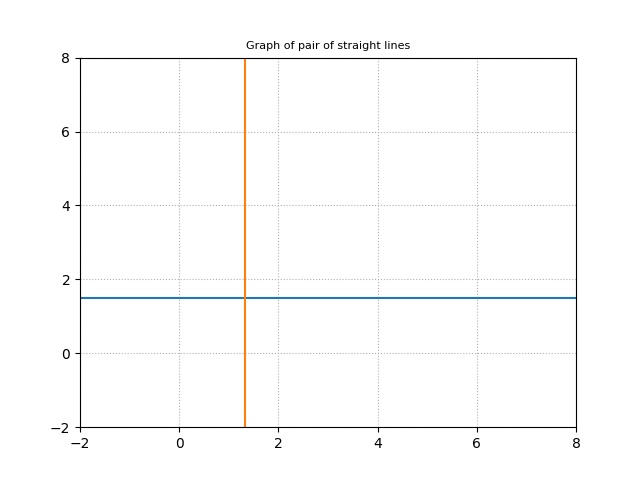
\includegraphics[width=\columnwidth]{./solutions/13/10/Figure_1.png}
\caption{Intersection of 2 lines}
\label{eq:solutions/13/10/Figure_1}
\end{figure}
substituting the values of $c_1$, $c_2$ and equation \eqref{eq:solutions/13/10/n1} and \eqref{eq:solutions/13/10/n2} to equation \eqref{eq:solutions/13/10/e1} and \eqref{eq:solutions/13/10/e2} we get equation of two straight lines.
\begin{align}
\implies \myvec{0&2}\vec{x} = \frac{8}{3}
\end{align}
\begin{align}
\myvec{3&0}\vec{x} = \frac{-9}{2}
\end{align}
Hence the equation of pair of straight lines are,
\begin{align}
\brak{\myvec{0&2}\vec{x}-\frac{8}{3}}\brak{\myvec{3&0}\vec{x} - \frac{-9}{2}} = 0
\label{eq:solutions/13/10/pair}
\end{align}
Hence, Plot of the equation \eqref{eq:solutions/13/10/pair} is shown in Figure.\ref{eq:solutions/13/10/Figure_1}
Now for value of k = 0 does not represent pair of straight lines.as,
\begin{align}
\mydet{\vec{V}} = \mydet{0&0\\0&0} \nless0 
\end{align} 
Hence, Plot of the equation $\myvec{-8&9}\vec{x} = 12$ is shown in figure \ref{eq:solutions/13/10/Figure_2},
\begin{figure}[ht!]
\centering
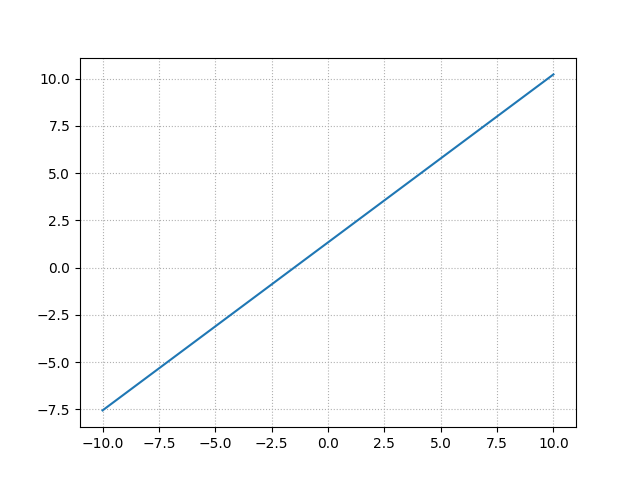
\includegraphics[width=\columnwidth]{./solutions/13/10/Figure_2.png}
\caption{Intersection of 2 lines}
\label{eq:solutions/13/10/Figure_2}
\end{figure}
